% EE6483 Mini Project (Option 1) 报告中文对照版。
% 内容与英文正式版 (report/main.tex) 逐节对应，仅供组内阅读，不作提交。
% 编译: 在 report/zh 目录下运行  latexmk -xelatex main_zh.tex
\documentclass[11pt,a4paper]{article}
\usepackage[margin=2.2cm]{geometry}
\usepackage[fontset=windows]{ctex}
\usepackage{amsmath,amssymb}
\usepackage{graphicx}
\usepackage{float}
\usepackage{booktabs}
\usepackage{tabularx}
\usepackage{array}
\usepackage{xcolor}
\color{black}
\usepackage{caption}
\usepackage{enumitem}
\usepackage{tikz}
\usetikzlibrary{positioning,arrows.meta,shapes.geometric,fit}
\usepackage[super,sort&compress]{natbib}
\usepackage[colorlinks=true,linkcolor=black,citecolor=black,urlcolor=black,filecolor=black]{hyperref}

\graphicspath{{../figures/}}
\setlist{itemsep=1pt,topsep=2pt,parsep=0pt,partopsep=0pt}
\setlist[itemize]{label=\textendash}
\usepackage[compact]{titlesec}
\titlespacing*{\section}{0pt}{1.4ex plus .4ex minus .2ex}{0.7ex plus .2ex}
\titlespacing*{\subsection}{0pt}{1.1ex plus .3ex minus .2ex}{0.5ex plus .1ex}
\titlespacing*{\paragraph}{0pt}{0.8ex plus .3ex minus .2ex}{0.8em}
\captionsetup{font=small,skip=4pt}
\renewcommand{\topfraction}{0.9}
\renewcommand{\bottomfraction}{0.8}
\renewcommand{\textfraction}{0.07}
\renewcommand{\floatpagefraction}{0.85}
\setcounter{topnumber}{3}
\setcounter{bottomnumber}{2}
\setcounter{totalnumber}{5}
\setlength{\textfloatsep}{8pt plus 2pt minus 2pt}
\setlength{\floatsep}{6pt plus 2pt minus 2pt}
\setlength{\intextsep}{6pt plus 2pt minus 2pt}
\newcolumntype{Y}{>{\raggedright\arraybackslash}X}
\renewcommand{\abstractname}{摘要}
\renewcommand{\refname}{参考文献}
\renewcommand{\figurename}{图}
\renewcommand{\tablename}{表}
\renewcommand{\appendixname}{附录}

\title{EE6483 人工智能与数据挖掘\\小项目（选题 1）：商品评论情感分析\\\large （中文对照版）}
\author{第 110 组 (Team 110)：MENG XIANGYU, WU DAYU, YIN JIYANG}
\date{2026 年 11 月}

\setlength{\parindent}{0pt}
\setlength{\parskip}{2pt plus 1pt}
\setlength{\emergencystretch}{2em}
\begin{document}
\vspace*{-1.8cm}
{\let\newpage\relax\maketitle}
\vspace{-0.6cm}

\section*{小组成员及分工}
\begin{table}[h]
\centering
\small
\begin{tabularx}{\textwidth}{l l l Y}
\toprule
姓名 & 学号 & 邮箱 & 贡献 \\
\midrule
MENG XIANGYU & G2607496E & \texttt{\footnotesize meng0106@e.ntu.edu.sg} & 公共代码（\texttt{common.py}、数据划分、评估）、TF-IDF 基线、噪声标签实验、资源与精度分析；第~\ref{sec:problem}、\ref{sec:data}、\ref{sec:formats}、\ref{sec:noise} 节；报告统稿。 \\
WU DAYU & G2603624F & \texttt{\footnotesize dayu002@e.ntu.edu.sg} & GloVe 特征、平均 GloVe + LR、BiLSTM 模型及调参；第~\ref{sec:recent}、\ref{sec:baseline}、\ref{sec:hparams}、\ref{sec:hotel} 节。 \\
YIN JIYANG & G2605135H & \texttt{\footnotesize jiyang002@e.ntu.edu.sg} & RoBERTa 微调、集成与最终提交、误差分析；第~\ref{sec:groups}、\ref{sec:models}、\ref{sec:results}、\ref{sec:analysis} 节；README。 \\
\bottomrule
\end{tabularx}
\end{table}
三位成员均为第~\ref{sec:recent} 节的文献表提供了论文，并交叉审阅了彼此负责的章节。

\begin{abstract}
我们研究商品评论的文档级情感分类（7{,}401 条带标签训练评论，85.4\% 为正面；1{,}851 条测试评论）。
在一个能避免重复文本泄漏的分组分层验证划分上，我们比较三种特征格式：稀疏 TF-IDF n-gram 加线性分类器、静态 GloVe 词向量加逻辑回归和 BiLSTM，以及微调的 RoBERTa-base 子词表示。
三次 RoBERTa 运行的平均在验证集上达到 0.962 的准确率和 0.927 的 Macro-F1，最好的 TF-IDF 模型分别为 0.930 和 0.857；BiLSTM 只与 TF-IDF 持平，训练时间却约为其 80 倍。
我们还讨论了向无标签酒店评论的迁移，并通过注入标签噪声的对照实验表明：在三种补救方法中，Confident Learning 式过滤最为可靠（20\% 对称噪声下 ROC-AUC 为 0.909，不做补救时为 0.837）。
\end{abstract}

\section{引言}\label{sec:intro}
情感分析判断一段文本的极性，商品评论是它最常见的应用之一。
本报告构建并评估把商品评论分为负面（0）或正面（1）的分类器。
训练集包含 7{,}401 条带标签评论，其中 85.4\% 为正面；测试集包含 1{,}851 条无标签评论。
这一任务同时具有训练数据有限、类别严重不平衡、文本带噪声且不规范等特点，因此特征格式的选择对精度和成本都很重要。

我们做出四点贡献。
(1) 我们定义了一个分组分层的验证划分，使重复的评论文本绝不会跨越划分，并将它用于所有模型，从而使各项得分可比。
(2) 我们在相同条件下比较三种成本递增的特征格式：稀疏 TF-IDF n-gram 加线性分类器，静态 GloVe 词向量加逻辑回归和 BiLSTM，以及子词序列加微调的 RoBERTa-base。
(3) 我们提交三次 RoBERTa 运行的平均结果，它在验证划分上达到 0.962 的准确率和 0.927 的 Macro-F1，并在一批人工标注的测试评论上分析其预测。
(4) 我们讨论该方法如何迁移到无标签的酒店评论，并通过标签翻转的对照实验说明噪声评分如何削弱它，以及三种补救方法中哪一种最有帮助。

第~\ref{sec:related} 节回顾相关文献。第~\ref{sec:data}--\ref{sec:hparams} 节描述数据、模型和参数设置；第~\ref{sec:results}--\ref{sec:formats} 节报告测试集结果、预测分析和特征格式的比较；第~\ref{sec:hotel} 节和第~\ref{sec:noise} 节分别讨论两种迁移场景，第~\ref{sec:conclusion} 节为结论。
表~\ref{tab:intro-map} 说明作业的每个问题在哪一节回答，附录~\ref{app:code} 说明如何复现结果。

\begin{table}[H]
\centering
\caption{作业各问题在报告中的对应位置。}
\label{tab:intro-map}
\small
\begin{tabular}{l l l}
\toprule
问题 & 主题 & 章节 \\
\midrule
(a) & 文献综述 & \ref{sec:related}（\ref{sec:problem}--\ref{sec:baseline}） \\
(b) & 特征格式与数据预处理 & \ref{sec:data} \\
(c) & 模型、结构、损失与训练 & \ref{sec:models} \\
(d) & 参数如何确定 & \ref{sec:hparams} \\
(e) & 测试集结果与 \texttt{submission.csv} & \ref{sec:results} \\
(f) & 分对与分错的样本 & \ref{sec:analysis} \\
(g) & 特征格式、资源与精度 & \ref{sec:formats} \\
(h) & 没有评分的酒店评论 & \ref{sec:hotel} \\
(i) & 评分带噪声的酒店评论 & \ref{sec:noise} \\
\bottomrule
\end{tabular}
\end{table}


%=====================================================================
\section{相关工作}\label{sec:related}
\subsection{问题定义、挑战与各类解决方案}\label{sec:problem}

\paragraph{问题定义。}
情感分析（又称观点挖掘）研究文本中人们表达的观点、情感和情绪的计算方法\cite{wankhade2022survey}。
一种常见的形式化方式把观点表示为五元组 $(e, a, s, h, t)$：实体 $e$、它的某个方面 $a$、针对该方面的情感 $s$、观点持有者 $h$ 以及时间 $t$。
本项目是这一定义下最简单的情形：\emph{文档级二分类极性判断}。
实体是所购买的商品，持有者是评论者，二者都是隐含的，每条评论对应整篇文档的一个标签。
给定评论 $x$，我们学习分类器 $f(x) \approx P(y{=}1 \mid x)$，其中 $y=1$ 表示正面、$y=0$ 表示负面，并按决策阈值 $\tau$ 预测 $\hat y = \mathbb{1}[f(x) \ge \tau]$。
中性或无关评论不在建模范围内。

\paragraph{分析粒度。}
情感可以在三个粒度上分析：
\begin{itemize}
  \item \emph{文档级}：每条评论一个标签，本项目即属于此类。
  \item \emph{句子级}：通常先做主观性过滤，再做极性分类。
  \item \emph{方面级}：基于方面的情感分析（ABSA）抽取``合身度''``面料''等方面，并分别给出极性\cite{zhang2023absa}。
\end{itemize}
相关任务使用更细的标签集合，例如 Stanford Sentiment Treebank 的五级量表，或情绪类别。

\paragraph{挑战。}
主要困难如下，每一条都结合了我们在数据中观察到的情况：
\begin{enumerate}
  \item \textbf{否定与转折。} ``not''``never''``but'' 等词会改变周围词语的极性。测试集中的 ``Not bad for just a shirt'' 里，``bad'' 单看是负面信号，但整条评论是轻度正面的。词袋模型丢失了解决这一问题所需的词序信息。
  \item \textbf{隐含情感、讽刺与反语。} 许多评论没有明确的观点词（``the seam came apart after one wash''），或者字面意思与真实意思相反。
  \item \textbf{极性混合。} 一条评论可能夸一个方面、批评另一个方面，文档标签取决于评论者更看重哪一方面。
  \item \textbf{领域依赖。} 词语的极性随领域变化。``Small'' 对酒店房间是负面、对手机常是正面，``unpredictable'' 对电影情节是正面、对汽车转向却是负面。因此在一类商品上训练的分类器迁移到另一类时性能会下降\cite{blitzer2007biographies}。
  \item \textbf{类别不平衡。} 商品评论以正面为主：训练集中 85.4\% 为正面、14.6\% 为负面。把所有评论都预测为``正面''就已经有 85.4\% 的准确率，因此除准确率外我们还报告 Macro-F1 和负类 F1。
  \item \textbf{噪声与非正式文本。} 评论中有错别字、俚语、表情符号，长度差异很大。训练集评论长度的中位数为 42 词，最长的有 1{,}066 词。当用星级作为标签时，部分标签与文本不符，这正是第~\ref{sec:noise} 节研究的问题。
\end{enumerate}

\paragraph{不同设定下的解决方案类型。}
表~\ref{tab:a1-settings} 按作业指出的三条轴线整理了常见方法；Wankhade 等人\cite{wankhade2022survey} 给出了更全面的近期综述。

\emph{有监督与无监督。}
有监督方法从带标签的评论中学习。它们包括：词袋特征上的朴素贝叶斯、最大熵和 SVM 分类器及其较强的 NB-SVM 变体；词向量上的卷积和循环网络；以及微调 BERT\cite{devlin2019bert} 及其后继的预训练 Transformer。
无监督的词典类方法不需要标签：
\begin{itemize}
  \item 根据短语与 ``excellent''``poor'' 等种子词的关联程度打分；
  \item 查询 SentiWordNet 等情感词典；
  \item 用 VADER 做基于规则的打分。
\end{itemize}
它们容易跨领域迁移，但准确率通常低于有监督模型。
介于两者之间的是弱监督方法：远程监督把表情符号或星级当作带噪标签，半监督方法对未标注评论做自训练。对大语言模型做零样本或少样本提示，在简单的二分类极性任务上有竞争力，但在细粒度和结构化情感任务上仍落后于微调模型\cite{zhang2023sentiment}。

\emph{封闭集与开放集。}
在封闭集设定下，每条测试评论都属于训练时的某个类别，这里即正面或负面。
在开放集设定下，测试输入可能来自训练中从未见过的类别：中性评论、垃圾信息、非评论文本或其他语言。
封闭集分类器仍然会把它们强行归为``正面''或``负面''。
开放集方法增加了拒识机制。DOC 把 softmax 换成一对多的 sigmoid，当没有任何类别足够自信时拒绝该输入；基于置信度的检测则标记最大 softmax 概率较低的输入。

\emph{有域偏移与无域偏移。}
当训练数据和测试数据来自同一分布时，使用标准的有监督学习即可。
在域偏移下，必须用源域（如图书）的带标签数据去服务无标签的目标域（如厨房电器）。方法包括：
\begin{itemize}
  \item 结构对应学习，通过共享的``枢轴''特征对齐领域特有的词\cite{blitzer2007biographies}；
  \item 学习领域不变表示的堆叠去噪自编码器；
  \item 域对抗训练（DANN）；
  \item 在目标领域文本上继续预训练语言模型。
\end{itemize}
这些方法是我们回答第~\ref{sec:hotel} 节问题的基础。

\begin{table}[!htbp]
\centering
\caption{不同设定下情感分类的解决方案类型。本项目的设定以 $\star$ 标出。}
\label{tab:a1-settings}
\small
\begin{tabularx}{\textwidth}{l Y Y}
\toprule
设定 & 典型方法 & 优点 / 局限 \\
\midrule
有监督 $\star$ & 词袋 + NB/LR/SVM；词向量上的 CNN/RNN；微调的 Transformer\cite{devlin2019bert} & 有领域内标注数据时最准确；需要标签，且与领域绑定。 \\
无监督 & 种子词关联；情感词典；规则方法（VADER） & 无需标签、可解释；忽略上下文、领域专有词和讽刺。 \\
弱监督 / 半监督 & 来自表情符号或评分的远程标签；自训练；大模型提示\cite{zhang2023sentiment} & 标签便宜、可大规模获得；标签含噪声（见第~\ref{sec:noise} 节）。 \\
\midrule
封闭集 $\star$ & 固定标签集上的 softmax & 简单；未见类别的输入被强行归入已知类别。 \\
开放集 & 一对多拒识（DOC）；置信度阈值 & 可以拒识中性或无关输入；需要额外阈值。 \\
\midrule
无域偏移 $\star$ & 标准的训练/验证/测试流程 & 验证集准确率能预测测试集准确率。 \\
有域偏移 & SCL 枢轴\cite{blitzer2007biographies}；去噪自编码器；DANN；领域自适应预训练 & 利用无标签的目标领域文本；收益取决于两个领域相距多远。 \\
\bottomrule
\end{tabularx}
\end{table}

\paragraph{我们的设定。}
本项目是\emph{有监督、封闭集、领域内}的设定。
训练评论和测试评论来自同一商品评论分布；1{,}851 条测试评论中甚至有 101 条与训练集原文完全相同。
数据类别不平衡，标签也可能含有一定噪声。
因此我们构建有监督分类器：以 TF-IDF 线性模型为基线，以序列模型和预训练语言模型作为改进；第~\ref{sec:baseline} 节说明了这一选择的动机。
我们用阈值调整和 Macro-F1 来处理类别不平衡。

%---------------------------------------------------------------------
\subsection{近期进展}\label{sec:recent}
表~\ref{tab:recent-sentiment} 涵盖领域自适应、情感感知的表示学习以及分布偏移下的评估。各论文报告的结果使用不同的基准和评测协议。

\begin{table}[!htbp]
\centering
\caption{情感分类与迁移方向的近期代表性工作。}
\label{tab:recent-sentiment}
\footnotesize
\renewcommand{\arraystretch}{1.0}
\begin{tabularx}{\textwidth}{@{}l >{\raggedright\arraybackslash}p{.16\textwidth}
  >{\raggedright\arraybackslash}p{.20\textwidth} Y Y@{}}
\toprule
年份 & 方法 & 数据 & 贡献 & 报告结果 \\
\midrule
2021 & UDALM\cite{karouzos2021udalm} & Amazon Reviews，12 个迁移方向 &
源域分类与目标域掩码语言建模联合训练 &
准确率 91.74\%，比此前对比方法高 1.11 个百分点。 \\
2022 & 基于记忆的对比学习\cite{tan2022memory} &
两个 Amazon 评论数据集和一个谣言数据集 &
面向未见领域的基于队列的有监督对比学习 &
优于被测试的领域自适应方法。 \\
2022 & 简单对比学习\cite{luo2022mere} &
Amazon Reviews 和 FDU-MTL &
用批内负样本在表示空间中分离不同类别 &
12 个 Amazon 迁移方向的平均准确率 90.39\%。 \\
2022 & 多领域目标情感分析\cite{toledoronen2022multi} &
用 Yelp 做自训练，3 个目标评估数据集 &
用跨领域的弱标注样本扩充训练 &
在各目标数据集上均有提升。 \\
2024 & SentiEval\cite{zhang2023sentiment} &
13 类情感任务共 26 个数据集 &
比较提示式大模型与针对任务训练的较小模型 &
简单分类任务对大模型更有利，细粒度结构化任务则不然。 \\
2024 & SoftMCL\cite{wang2024softmcl} &
句子级和方面级情感及其他情感类任务 &
预训练时使用软效价和动量队列 &
在多个情感任务上都有收益。 \\
2025 & 合成指令\cite{zhao2025instruction} &
12 个情感基准，包括 Amazon、Yelp、IMDb &
不使用带标签的评论实例来构造指令样本 &
比更复杂的指令微调方法高 5.1 个点。 \\
2025 & BESSTIE\cite{srirag2025besstie} &
三种英语变体的 Google Place 和 Reddit 文本 &
跨英语变体测试情感和讽刺 &
在印度英语上性能下降，尤其是讽刺。 \\
\bottomrule
\end{tabularx}
\end{table}

领域自适应方面的研究表明，即使没有评分，也可以在训练中使用酒店文本。跨变体评估和大模型对比还提示，在测试迁移效果时应保留一份目标领域的留出样本。对于本项目的商品评论任务，我们先在同一划分上比较稀疏词汇特征模型和稠密词向量模型，再对迁移问题下结论。

%---------------------------------------------------------------------
\subsection{代表性研究组}\label{sec:groups}
南洋理工大学 Erik Cambria 的研究组研究如何利用常识知识帮助系统判断文本的情感并解释其决策。SenticNet 7 和 SenticNet 8 展示了这一方向的发展：第一篇的重点是构建把不同表达关联到共享概念的知识库，第二篇在此基础上进一步考察这些概念在句子中的含义。

\paragraph{SenticNet 7（2022）。}
Cambria 等人\citep{cambria2022senticnet} 用 XLNet 提出在上下文中可能表达相近含义的词和短语。基于 ConceptNet 中情绪概念链接的相似度度量，用来区分那些在上下文中看似相近、实则情感不同的表达。得到的知识库既包含单词也包含短语。例如，它把 ``dead right'' 当作有独立含义的短语，因此单词 ``dead'' 本身并不决定它的情感。

作者在包括 Amazon 评论和 IMDb 评论在内的十个数据集上，把 SenticNet 7 与 20 个情感词典作了比较。他们把其性能的一部分归因于更广的词汇覆盖，因为其他词典的常见错误来源是词条缺失。讽刺，以及对不同对象表达相反观点的句子，仍会造成错误。更大的词表能帮助系统识别更多表达，而判断哪个观点对应哪个对象仍是另一个独立问题。

\paragraph{SenticNet 8（2024）。}
SenticNet 8 把常识知识库与一个层次注意力网络结合，后者找出与情感判断最相关的词元\citep{cambria2024senticnet}。它的文本处理流程从统一措辞开始，到把含义相近的表达归组，再到描述这些表达所指的情境。论文用几种描述购买手机的说法作为例子：``buy a phone'' 和 ``pay for a phone'' 都可以表示为手机所有者发生了变化。这个例子使中间表示的作用更容易理解。

在 Sentiment140 极性任务上，SenticNet 8 的准确率为 88.80\%，同一篇论文中的 RoBERTa 基线为 85.07\%。测试文本是推文，因此把该方法用于商品评论还需要单独评估。

\paragraph{与商品评论的关系。}
第~\ref{sec:analysis} 节中的评论 1123 说明了观点对象的问题。评论者描述旧塑料行李牌开裂、断掉，然后解释为什么新的皮质行李牌是更好的选择。最初的 RoBERTa 集成预测为负面，而最终的人工标签为正面。如果能把``旧牌子的损坏''和``对新牌子的推荐''分别关联起来分析，就可能保留对这条评论至关重要的区别。SenticNet 是否能正确分类这个例子，仍是一个需要在同一数据上直接对比的开放问题。

%---------------------------------------------------------------------
\subsection{基线的选择与改进动机}\label{sec:baseline}
词级 TF-IDF 加逻辑回归是合适的基线。它能高效处理稀疏的评论向量，其系数还能显示哪些特征驱动了预测。二元组可以捕捉 \emph{not good} 这样的局部短语。更长的上下文，包括后一个分句推翻前面观点的情形，仍然难以用局部特征处理。精确的词项匹配对未见词的覆盖也有限。

我们在同一个分组划分上评估两种扩展。第一种是平均静态词向量（如 Word2Vec 或 GloVe）\cite{mikolov2013efficient,pennington2014glove}，每条评论得到一个稠密的 300 维表示；再用逻辑回归分类器检验这一表示是否保留了有用的情感信息。第二种是 BiLSTM，它保留词序，学习正向和反向表示后再池化。Transformer 这条线则评估上下文相关的子词表示。由于特征表示和分类器在不同模型线之间都会改变，得分差异反映的是每个完整系统的性能。

在阈值 0.5 时，验证集 Macro-F1 分别为：TF-IDF + LR 0.8451，平均 GloVe + LR 0.7623，三个 seed 的 BiLSTM 0.8524。在本实验中，序列模型优于平均向量模型，它的得分比 TF-IDF + LR 高 0.0072。该比较只基于单个验证划分。

%=====================================================================
\section{数据与特征表示}\label{sec:data}

\subsection{特征格式与处理流程}
我们比较三种成本递增的特征格式，每条模型线对应一种，以便第~\ref{sec:formats} 节能直接衡量这种权衡：
\begin{enumerate}
  \item \textbf{带 TF-IDF 权重的稀疏 n-gram 词袋}，供线性分类器使用；
  \item \textbf{静态预训练词向量}（300 维 GloVe\cite{pennington2014glove}），供平均词向量分类器和 BiLSTM 使用；
  \item \textbf{输入预训练 Transformer 的子词序列}（RoBERTa-base），其上下文表示被端到端地微调。这是我们最终模型使用的格式。
\end{enumerate}
图~\ref{fig:b-pipeline} 概括了整个流程。三种格式共享下面描述的读取、检查、划分和清洗步骤。

\begin{figure}[!htbp]
\centering
\begin{tikzpicture}[
  node distance=4mm and 6mm,
  box/.style={draw, rounded corners=2pt, align=center, font=\footnotesize, minimum height=8mm, text width=27mm, fill=gray!8},
  fbox/.style={box, text width=36mm, fill=gray!20},
  arr/.style={-{Stealth[length=2mm]}, thick}]
\node[box] (load) {读取 \texttt{train.json}\\(7{,}401) / \texttt{test.json} (1{,}851)};
\node[box, right=of load] (audit) {检查：类别不平衡、\\长度、重复};
\node[box, right=of audit] (split) {分组分层划分\\训练 5{,}909 / 验证 1{,}492};
\node[box, right=of split] (clean) {轻量清洗\\（HTML、空白）};
\node[fbox, below=9mm of audit, xshift=-6mm] (tfidf) {\textbf{TF-IDF}：小写，词 1--2-gram（+ 字符 2--5-gram），次线性 tf，L2 $\rightarrow$ 稀疏 $x\in\mathbb{R}^{50\text{k}}$};
\node[fbox, right=of tfidf] (glove) {\textbf{GloVe}：小写词元 $\rightarrow$ 词表编号 $\rightarrow$ 300 维向量（取平均或保留序列，$L\le256$）};
\node[fbox, right=of glove] (bpe) {\textbf{RoBERTa}：保留大小写的字节级 BPE $\rightarrow$ 编号 + 掩码，$L\le256$};
\draw[arr] (load) -- (audit);
\draw[arr] (audit) -- (split);
\draw[arr] (split) -- (clean);
\draw[arr] (clean.south) |- ++(0,-4mm) -| (tfidf.north);
\draw[arr] (clean.south) |- ++(0,-4mm) -| (glove.north);
\draw[arr] (clean.south) -- ++(0,-4mm) -| (bpe.north);
\end{tikzpicture}
\caption{数据预处理流程。所有向量化器、词表和模型都只在训练部分上拟合；验证集只用于模型选择，测试集只用于生成最终预测。}
\label{fig:b-pipeline}
\end{figure}

\subsection{数据检查}
两个文件都按 JSON 表格读取。
训练集有 7{,}401 条评论，带二分类标签（6{,}319 条正面，1{,}082 条负面）。测试集有 1{,}851 条无标签评论。没有缺失或空评论。
评论长度差异很大：中位数为 42 词，75\% 的评论不超过 70 词，97\% 不超过 178 词，最长的有 1{,}066 词。
我们还检查了重复情况，比较时先统一转小写并合并空白：
\begin{itemize}
  \item 训练集中有 154 段不同的文字出现多次，共涉及 373 行，同一段文字的所有副本标签一致；
  \item 有 101 条测试评论与某条训练评论完全相同；
  \item 有 21 条测试评论与另一条测试评论重复。
\end{itemize}

\subsection{分组分层的验证集划分}
所有模型都在同一个共享验证集上调参。
如果随机划分重复评论，同一评论的副本会同时出现在两边，验证分数就会部分反映模型的记忆能力。
因此我们按标准化后的文本给各行分组，取 5 折 \texttt{StratifiedGroupKFold}（seed 42）的第 0 折。
由此得到 5{,}909 条训练评论和 1{,}492 条验证评论。验证集含 218 条负面评论（14.6\%，与全集比例相同），没有任何文本同时出现在两侧。
训练部分内部的交叉验证，包括校准 SVM 所用的内部折，使用同样的分组方式。
测试集只用于生成 \texttt{submission.csv}。

\subsection{文本清洗}
我们对 HTML 实体做反转义，合并连续空白，并去掉首尾空格。
我们\emph{有意不}做以下处理：
\begin{itemize}
  \item 去除停用词，因为标准停用词表包含 ``not''``no''``but''，这些词带有情感信息；
  \item 词干提取，或去掉 ``!''``?'' 等标点。
\end{itemize}
TF-IDF 和 GloVe 使用小写文本；RoBERTa 的分词器区分大小写，所以保留原始大小写。

\subsection{TF-IDF 特征（L1）}
分词使用的模式会保留单字符词元（如 ``don't'' 里的 ``t''）以及 ``!'' 和 ``?''。
我们提取一元组和二元组；二元组能捕捉 ``not good''``not worth'' 这样的短否定。
评论 $d$ 中的每个词项 $t$ 使用次线性词频和平滑的逆文档频率加权，
\begin{equation}
  w_{t,d} = \bigl(1 + \log \mathrm{tf}_{t,d}\bigr)\cdot\Bigl(\log\frac{1+N}{1+\mathrm{df}_t} + 1\Bigr),
\end{equation}
其中 $N$ 为训练评论数，$\mathrm{df}_t$ 为包含 $t$ 的评论数。随后对每条评论的向量做 L2 归一化。
向量化器只在训练行上拟合。
我们用分组 5 折交叉验证调了三项设置：
\begin{itemize}
  \item 最小文档频率（1、2 或 3）；
  \item 词表上限（1 万、3 万、5 万或不限）；
  \item 是否追加字符 2--5-gram（可以吸收拼写错误）。
\end{itemize}
最终选定的表示有 50{,}000 个词级 1--2-gram 特征。它非常稀疏：平均每条评论 86 个非零项，密度 0.17\%。

\subsection{静态词向量（L2）}
L2 的分词器对文本做小写和反转义，保留缩写以及标点词元 \texttt{!} 和 \texttt{?}，最多保留 256 个词元。
词表只在训练部分上构建，最小词频为 2，并带有 \texttt{<pad>} 和 \texttt{<unk>} 两个特殊条目。在 6{,}796 个普通训练词表条目中，有 6{,}359 个在 300 维 \texttt{glove.6B} 表\cite{pennington2014glove} 中有向量。
在验证集上，有 3.17\% 的词元出现被映射为 \texttt{<unk>}，应用词表后有 4.95\% 没有可用的预训练向量。
平均 GloVe 只对有向量的词求平均。BiLSTM 对词表内但缺少 GloVe 向量的条目以及共享的未知词条目使用随机初始向量。填充位置不参与两个方向的计算，也不参与池化统计。

\subsection{预训练 Transformer 的子词序列（L3）}
清洗之后，评论保留原始大小写。RoBERTa 的字节级 BPE 分词器把文本转成词元编号，并加上 \texttt{<s>} 和 \texttt{</s>}。256 个词元的上限包含这些特殊词元。评论过长时，分词器保留文本开头部分。每个批次按其中最长的序列补齐，注意力掩码区分输入词元和填充。第~\ref{sec:models} 节说明模型如何使用第一个词元的表示做分类。

\subsection{标签与类别不平衡}
标签按原样使用（0 = 负面，1 = 正面）。
每个模型输出 $P(y{=}1\mid x)$。我们同时报告阈值为 0.5 时的指标，以及在验证集上调过阈值后的指标：一个使准确率最大（$\tau_{\mathrm{acc}}$，用于提交），一个使 Macro-F1 最大（$\tau_{\mathrm{F1}}$）。
RoBERTa 的运行使用不加权的交叉熵。第~\ref{sec:hparams} 节说明了对其他模型评估过的参数设置。

%=====================================================================
\section{模型}\label{sec:models}

\subsection{TF-IDF 分类器}
三个 TF-IDF 分类器的输入是第~\ref{sec:data} 节描述的稀疏 n-gram 向量。逻辑回归把特征的加权和映射为正类概率。线性 SVM 给出间隔分数，再通过在训练部分内的分组折上做 sigmoid 校准转成概率。Complement Naive Bayes 用另一类评论来估计每个类别的特征权重，并带有加性平滑。特征和分类器的设置由训练部分内的分组五折交叉验证选出。每个选定的模型随后在 5{,}909 条评论上拟合，并在 1{,}492 条共享验证集评论上评估。在预测测试集时，TF-IDF 向量化器和分类器都在全部 7{,}401 条带标签评论上重新拟合。

\subsection{GloVe 词向量与 BiLSTM}
平均词向量分类器对评论中各词元可用的 GloVe 向量求平均。如果没有任何词元有预训练向量，该评论用零向量表示。得到的 300 维特征输入带正则化的逻辑回归分类器。

BiLSTM 使用同一个训练词表来初始化大小为 $V \times 300$ 的嵌入矩阵，其中 $V$ 为词表大小。没有预训练向量的条目用均值为零、标准差为 0.05 的高斯分布初始化，填充行固定为零。输入是形状为 $B \times L$ 的整数词元编号批次，其中 $B$ 为批大小，$L \leq 256$。

\begin{figure}[!htbp]
\centering
\begin{tikzpicture}[
  node distance=3mm,
  modelblock/.style={
    draw, rounded corners, align=center,
    text width=.69\linewidth, inner sep=5pt
  }
]
\node[modelblock] (tokens) {词元编号 $[B,L]$};
\node[modelblock, below=of tokens] (embed)
  {GloVe 初始化的嵌入 $[B,L,300]$};
\node[modelblock, below=of embed] (recur)
  {两层双向 LSTM $[B,L,2H]$};
\node[modelblock, below=of recur] (pool)
  {带掩码的最大池化与平均池化，拼接 $[B,4H]$};
\node[modelblock, below=of pool] (out)
  {Dropout 与线性分类器 $[B,2]$};

\draw[-{Latex}] (tokens) -- (embed);
\draw[-{Latex}] (embed) -- (recur);
\draw[-{Latex}] (recur) -- (pool);
\draw[-{Latex}] (pool) -- (out);
\end{tikzpicture}
\caption{GloVe 初始化的 BiLSTM。$H$ 表示每个方向的隐藏维度。}
\label{fig:bilstm}
\end{figure}

在每一层中，反向 LSTM 只翻转序列的有效部分。两种池化都忽略填充。最大池化保留每个通道上最强的激活，平均池化则概括有效位置的状态。两个池化向量拼接后，给分类器提供 $4H$ 个特征，即 $H = 128$ 时为 512 个。BiLSTM 用 Adam 和交叉熵训练。在加权版本中，类别 $j$ 的损失权重为 $n/(2n_j)$，其中 $n$ 为训练评论数，$n_j$ 为该类评论数。最佳 epoch 按阈值 0.5 时的验证集 Macro-F1 选择。Softmax 给出正类概率，验证集和测试集的概率在 seed 42、43、44 之间取平均。

\subsection{RoBERTa-base}
\paragraph{输入与分类器。}
经过第~\ref{sec:data} 节所述的轻量清洗后，每条评论保留原始大小写。RoBERTa 分词器把文本切成子词，并把序列限制在 256 个词元以内（含特殊词元）。更长的序列从末尾截断。在每个批次内，较短的序列补齐到与最长序列等长，注意力掩码区分输入词元与填充。

编码器在每个词元位置输出 768 维表示。分类头读取第一个词元 \texttt{<s>} 处的表示：先经过一个带 tanh 激活的全连接层，训练时该层前后各有一个 dropout，最后的线性层为每个类别输出一个分数。Softmax 把两个分数转成概率，保留正类概率用于预测。

\begin{figure}[!htbp]
\centering
\begin{tikzpicture}[
  node distance=6mm,
  box/.style={
    draw, rounded corners=2pt, align=center, font=\footnotesize,
    minimum height=21mm, inner xsep=2mm, fill=gray!8
  },
  model/.style={box, fill=gray!20},
  arr/.style={-{Stealth[length=2mm]}, thick}
]
\node[box, text width=25mm] (input) {
  \textbf{分词后的评论}\\
  词元编号与掩码\\
  $B \times L$
};
\node[model, text width=30mm, right=of input] (encoder) {
  \textbf{RoBERTa-base}\\
  上下文向量\\
  $B \times L \times 768$
};
\node[model, text width=47mm, right=of encoder] (head) {
  \textbf{分类头}\\
  首词元向量：$B \times 768$\\
  Dropout $\to$ 全连接 + \texttt{tanh}\\
  Dropout $\to$ 线性层 ($768 \to 2$)
};
\node[box, text width=24mm, right=of head] (output) {
  \textbf{Softmax}\\
  正类\\
  概率
};

\draw[arr] (input) -- (encoder);
\draw[arr] (encoder) -- (head);
\draw[arr] (head) -- (output);
\end{tikzpicture}
\caption{用于评论分类的 RoBERTa-base 结构。$B$ 为批大小，$L \leq 256$ 为批内补齐后的序列长度。分类头使用编码器在首词元 \texttt{\textless s\textgreater} 处的输出。}
\label{fig:c-roberta}
\end{figure}

\paragraph{微调。}
编码器和分类头在共享划分的 5{,}909 条训练评论上一起微调。三次最终运行都使用 1 个 epoch、FP32 精度、批大小 4 以及不加权的交叉熵。AdamW 的权重衰减为 0.01。学习率在前 10\% 的训练步中升到 $2 \times 10^{-5}$，然后线性衰减到零。第~\ref{sec:hparams} 节说明了我们如何选定这一调度。

\paragraph{预测。}
三次运行的数据划分和训练设置保持不变，随机种子分别为 42、43、44。对每条评论，先把三个正类概率取平均，再应用决策阈值。第~\ref{sec:results} 节说明阈值如何在验证集上选定，并给出得到的测试集预测。

%=====================================================================
\section{参数选择}\label{sec:hparams}

\paragraph{稀疏基线。}
稀疏模型在 5{,}909 条训练评论内使用分组五折交叉验证。TF-IDF 网格覆盖最小文档频率、词表上限和可选的字符特征，它们控制着``覆盖罕见表达''与``特征数量''之间的权衡。逻辑回归使用 $C=10$ 和平衡类别权重，特征为 50{,}000 个词的一元组和二元组。校准后的线性 SVM 选择 $C=1$、不加类别权重，ComplementNB 选择 $\alpha=0.1$ 和 10{,}000 个特征。

\paragraph{静态词向量模型。}
对于平均 GloVe，我们比较 $C\in\{0.1,1,10\}$，并分别在加和不加平衡类别权重的情况下测试。在统一阈值 0.5 下，$C=10$ 且加平衡权重的设置 Macro-F1 最高（0.7623）。不加权的对应设置 Macro-F1 为 0.7598、准确率为 0.8988，而加权后准确率为 0.8539。加权后负类 F1 更高（0.6148 对 0.5770），这解释了尽管准确率有所损失仍选择它的原因。BiLSTM 从 Adam、学习率 $10^{-3}$、每个方向隐藏维度 128、dropout 0.3、可训练嵌入和普通交叉熵开始。依次搜索的顺序为：学习率（$10^{-3}$ 或 $5\times10^{-4}$）、隐藏维度（64、128 或 256）、dropout（0.3 或 0.5）、是否冻结嵌入，最后是类别加权。这样控制了成本，并让每次比较都围绕当前最优配置展开；要估计各设置之间的交互效应，则需要因子设计的搜索。
学习率控制步长，dropout 减少过拟合，冻结嵌入用来检验源监督信号是否受益于更新 GloVe。类别加权在训练中改变梯度，而阈值调整在训练后改变工作点。每次运行使用 64 的批大小、1.0 的梯度裁剪、最多 10 个 epoch，早停耐心值为两个 epoch。

候选配置按阈值 0.5 时的验证集 Macro-F1 排序。选定的 BiLSTM 配置用 seed 42、43、44 重复运行。我们用标准差描述运行之间的波动。由于同一个验证折也用于指导调参和早停，这些是模型选择分数。无标签的商品测试集只用于预测。
随后对每个模型，在验证集概率上分别拟合准确率阈值和 Macro-F1 阈值。

顺序搜索共运行了七种配置，之后进行三次最终拟合。选定的学习率为 $0.001$，每个方向宽度 128，dropout 0.3，嵌入可训练，使用普通交叉熵。单个 seed 的 Macro-F1 为 $0.8383\pm0.0050$（均值和总体标准差）。三个 seed 的概率平均在阈值 0.5 下的 Macro-F1 为 0.8524。验证集选出的阈值为 $\tau_{\mathrm{acc}}=0.500$ 和 $\tau_{\mathrm{F1}}=0.500$。各配置及其得分记录在项目代码库中（见附录~\ref{app:code}）。

\paragraph{Transformer。}
我们最初用 AdamW 对 RoBERTa-base 微调 1 个 epoch，学习率恒定为 $2\times10^{-5}$，权重衰减 0.01。使用不加权的交叉熵、批大小 4、最大序列长度 256 个词元和 FP32 精度。在阈值 0.5 下，seed 42 和 43 的验证集 Macro-F1 分别为 0.897 和 0.884。Seed 44 得分为 0.461，并把每条验证评论都判为正面。

在原设置下重复运行 seed 44 得到了同样的 Macro-F1。在相同的恒定学习率下把训练延长到两个 epoch，第二个 epoch 结束时 Macro-F1 仍为 0.461。这种 seed 之间的差异说明，原来的微调设置对随机性敏感。随机种子同时影响分类头的初始化和训练样本的顺序，因此我们的运行无法分离这两个因素各自的作用。

我们回到 1 个 epoch，并改变了学习率调度：学习率在前 10\% 的训练步中升到 $2\times10^{-5}$，然后线性衰减到零。Seed 44 在同一阈值下的 Macro-F1 提高到 0.914。随后我们用同样的调度重跑了 seed 42 和 43，使三次运行都使用相同的设置。三个 seed（42、43、44）最终的 Macro-F1 分别为 0.920、0.910 和 0.914。在后面的章节中，\emph{初始集成}指三次恒定学习率运行的平均，\emph{最终集成}指三次采用预热的运行的平均。

%=====================================================================
\section{测试集结果}\label{sec:results}

\paragraph{最终模型。}
我们对三次采用 10\% 预热和线性衰减训练的 RoBERTa-base 的正类概率取平均。在阈值 0.5 下，单次运行 Macro-F1 的总体标准差，从原调度下的 0.203降到这三个 seed 之间的 0.004。在验证集上，最终的 RoBERTa 集成在选定阈值后的 Macro-F1 为 0.927。75\% RoBERTa 加 25\% TF-IDF + SVM 的混合在各自选阈值后为 0.926，所以我们使用 RoBERTa 集成作为提交结果。

\paragraph{决策阈值。}
在 1{,}492 条有标签的验证评论上，对 RoBERTa 集成所评估的阈值中，0.590 使准确率（0.962）和 Macro-F1（0.927）都最高。我们把同一阈值用于测试集：平均正类概率不低于 0.590 的评论标为 1，其余标为 0。

\paragraph{测试集预测。}
表~\ref{tab:e-dist} 给出 1{,}851 条无标签测试评论的预测标签分布。

\begin{table}[!htb]
\centering
\caption{1{,}851 条测试评论的预测标签分布。}
\label{tab:e-dist}
\small
\begin{tabular}{lrr}
\toprule
预测标签 & 评论数 & 占比 \\
\midrule
正面 (1) & 1{,}568 & 84.71\% \\
负面 (0) & 283 & 15.29\% \\
\midrule
合计 & 1{,}851 & 100.00\% \\
\bottomrule
\end{tabular}
\end{table}

文件 \texttt{submission.csv} 包含 \texttt{reviews} 和 \texttt{predictions} 两列，顺序与原测试集一致。

%=====================================================================
\section{预测分析}\label{sec:analysis}

\paragraph{测试样本与标注。}
本节的误差分析使用最初的 RoBERTa 集成，即采用恒定学习率训练、在阈值 0.680 下评估的版本。排除 101 条文本也出现在训练集中的测试评论后，我们选了 40 条评论做人工标注。其中 15 条最接近最初 RoBERTa 的决策阈值，15 条取自该集成与 TF-IDF + SVM 预测不一致的评论，10 条从剩余评论中随机抽取。两名成员独立标注了全部 40 条，其中 38 条一致（95\%），第三名成员裁定了两条分歧。

\paragraph{正确与错误的预测。}
在抽样的 40 条评论中，RoBERTa 与最终人工标签一致的有 31 条（0.775）。样本有意包含了接近决策阈值的评论和模型之间存在分歧的评论，所以这一准确率只适用于被选中的评论。在同样这 40 条评论上，第~\ref{sec:results} 节所述的最终 RoBERTa 集成与人工标签一致的有 34 条（0.850）。

RoBERTa 正确分类了评论 274 和 99。评论 274 中，评论者指出了这件衣服的一个局限，但仍推荐它用于在衣服下面修饰身形。这一推荐支持了正面标签。评论 99 中，评论者起初喜欢这件文胸的版型和支撑，但钢圈最终戳穿了出来。这种故障支持负面标签，尽管前面有过称赞。

RoBERTa 把评论 549 判为正面，尽管评论者反映靴子的搭扣断了，并询问能否退货。它把评论 1123 判为负面。在那条评论中，评论者描述的开裂和断掉指的是旧塑料行李牌，而评论者对新的皮质行李牌是满意的，这才是被评价的商品。

\paragraph{验证集上的错误。}
在 1{,}492 条共享验证评论上，TF-IDF + SVM、BiLSTM 和 RoBERTa 分别分错 109、104 和 69 条。三个模型都分错的 30 条评论中，有 12 条含有混合情感。RoBERTa 正确分类了 66 条 SVM 分错的评论，其中 9 条被归为涉及上下文或否定。例如验证评论 523 中，短语 ``not disappointed'' 表示认可，评论者最后还给出了推荐。

%=====================================================================
\section{特征格式、精度与资源}\label{sec:formats}

特征格式决定两件事：到达分类器的信息是什么（只有词的身份、词的相似性，还是词在上下文中的含义），以及获得这些信息需要多少计算和内存。
我们先从一般角度比较三种格式（表~\ref{tab:g-qual}），然后报告在本数据集上的实测结果（表~\ref{tab:g-measured}），最后在 TF-IDF 这条线内部单独考察特征维度的影响（表~\ref{tab:g-dims}）。

\begin{table}[!htbp]
\centering
\caption{本项目使用的三种特征格式的比较。}
\label{tab:g-qual}
\small
\begin{tabularx}{\textwidth}{l Y Y Y}
\toprule
 & TF-IDF n-gram（L1） & 静态 GloVe 词向量（L2） & 上下文子词，RoBERTa（L3） \\
\midrule
表示 & 稀疏，每个 n-gram 一维（这里 5 万维，0.17\% 非零） & 稠密，每个词元 300 维；取平均或按序列 & 稠密，每个子词词元 768 维，依赖上下文 \\
词序 / 上下文 & 仅通过二元组获得局部信息 & 平均：无。BiLSTM：按序列学习 & 对 256 个词元做完整自注意力 \\
相近词 & 维度互不相关（``great'' 与 ``excellent''） & 在向量空间中接近 & 接近，且能依据上下文消歧 \\
未登录词 & 被丢弃（占验证集词元的 2.1\%、词类型的 24\%） & \texttt{<unk>} 或随机向量（验证集词元 3.2\% 为 \texttt{<unk>}；5.0\% 没有预训练向量） & 无：未知词会被拆成子词 \\
可训练参数 & 约为维度数 $+\,1$（5 万） & 平均+LR：301。BiLSTM：290 万（含嵌入表） & 约 1.25 亿 \\
硬件 / 训练成本 & CPU，数秒 & CPU，数分钟（BiLSTM） & GPU，数分钟到数小时 \\
内存 & 几 MB 的稀疏矩阵 & 嵌入表 $V\times300$（完整 GloVe 文件约 1\,GB） & 约 0.5\,GB 权重加激活值 \\
可解释性 & 高：每个 n-gram 一个权重 & 低 & 低（需要归因方法） \\
所需数据量 & 中等；数据越多越有利 & 较少，得益于预训练向量 & 达到同样精度所需最少；知识来自预训练迁移 \\
\bottomrule
\end{tabularx}
\end{table}

\begin{table}[!htbp]
\centering
\caption{在共享验证集（1{,}492 条评论，其中 218 条负面）上测得的精度与资源占用。训练时间为每次运行的时间（神经模型为每个 seed），不含加载数据和预训练权重的时间。TF-IDF 的运行是确定性的。神经模型对 seed 42/43/44 的概率取平均。RoBERTa 一行使用三次采用 10\% 预热和线性衰减训练的运行，其训练时间为三次运行的平均值，峰值 GPU 显存为三次中的最大值。各条线的硬件不同：TF-IDF 在 AMD 笔记本 CPU（16 线程）上，GloVe 模型在 9 线程 x86-64 CPU 上，RoBERTa 在 NVIDIA RTX 3070 Ti Laptop GPU 上。}
\label{tab:g-measured}
\footnotesize
\setlength{\tabcolsep}{3pt}
\begin{tabular}{l r r r r r r r}
\toprule
模型 & 特征维度 & 参数量 & Acc@0.5 & Acc@$\tau_{acc}$ & Macro-F1@$\tau_{f1}$ & 训练 (s) & 峰值内存 (MiB) \\
\midrule
TF-IDF + LR            & 50{,}000 & 50{,}001  & 0.924 & 0.928 & 0.851 & 1.5 & 122 \\
TF-IDF + SVM     & 50{,}000 & 150{,}009$^{\dagger}$ & 0.929 & 0.930 & 0.857 & 2.8 & 150 \\
TF-IDF + ComplementNB  & 10{,}000 & 20{,}000  & 0.910 & 0.926 & 0.857 & 1.2 & 155 \\
平均 GloVe + LR & 300 & 301 & 0.854 & 0.899 & 0.788 & 0.06 & 351 \\
GloVe + BiLSTM & 300/词元 & 2{,}876{,}010 & 0.930 & 0.930 & 0.852 & 121.6 & 1{,}112 \\
RoBERTa-base & 768/词元 & 124{,}647{,}170 & 0.959 & 0.962 & 0.927 & 113.1 & 2{,}434$^{\S}$ \\
\bottomrule
\end{tabular}\\[2pt]
\footnotesize $^{\dagger}$三个校准后的 SVM，每个内部校准折一个，各有自己的权重向量。
$^{\S}$峰值 GPU 显存；其余各行报告的是 CPU 进程内存。
\end{table}

\begin{table}[!htbp]
\centering
\caption{TF-IDF 维度的影响。分类器固定（LR，$C{=}10$，平衡类别权重），在训练部分上训练，在验证集上评估。}
\label{tab:g-dims}
\footnotesize
\setlength{\tabcolsep}{3pt}
\begin{tabular}{l r r r r r r}
\toprule
特征 & 维度 & 每条评论非零项数 & 矩阵 (MB) & 向量化 + 拟合 (s) & Macro-F1@0.5 & AUC \\
\midrule
词 1--2-gram，前 1k   & 1{,}000   & 45  & 3.1  & 1.2 & 0.811 & 0.930 \\
词 1--2-gram，前 5k   & 5{,}000   & 63  & 4.3  & 1.2 & 0.840 & 0.946 \\
词 1--2-gram，前 10k  & 10{,}000  & 70  & 4.8  & 1.1 & 0.845 & 0.949 \\
词 1--2-gram，前 30k  & 30{,}000  & 81  & 5.5  & 1.3 & 0.850 & 0.951 \\
词 1--2-gram，前 50k  & 50{,}000  & 86  & 5.8  & 1.3 & 0.845 & 0.950 \\
词 1--2-gram，全部      & 123{,}515 & 98  & 6.7  & 1.2 & 0.846 & 0.951 \\
\quad + 字符 2--5-gram（全部） & 174{,}735 & 649 & 43.9 & 6.3 & 0.858 & 0.952 \\
\bottomrule
\end{tabular}
\end{table}

\paragraph{同一种格式内的维度。}
表~\ref{tab:g-dims} 显示出明显的收益递减。
把 TF-IDF 词表从 1k 扩大到 30k 个 n-gram，Macro-F1 从 0.811 升到 0.850，AUC 从 0.930 升到 0.951。超过 30k 后收益停止：保留全部 123k 个 n-gram，AUC 的变化不到 0.001。
由于表示是稀疏的，成本随名义维度增长得很慢。每条评论只激活 45--98 个条目，训练矩阵始终不到 7\,MB。
追加字符 2--5-gram 是个例外：它使每条评论的非零项数增加约 7 倍（649 对 98），矩阵大小增加 6.5 倍，训练时间增加 5 倍。
验证集 Macro-F1 上升约 0.01，但分组 5 折交叉验证显示没有收益（加字符 n-gram 为 0.8514，不加为 0.8515）。
对只有 218 条负面样本的划分来说，0.01 的 Macro-F1 差异在噪声范围内，因此选择了更便宜的纯词级表示。

\paragraph{跨格式比较：精度。}
三种格式暴露的语言结构多少不同。
TF-IDF 已经达到 0.928--0.930 的准确率，因为大多数评论含有强烈、明确的观点词。
LR 中权重最大的特征符合直觉：负面评论是 ``disappointed''``uncomfortable''``returned''``poor''，正面评论是 ``great''``comfortable''``perfect''``love''。
然而，一元组 ``not'' 本身得到的权重最负。因此 ``not bad'' 只得到一个很小的正二元组权重（+0.59），几乎抵不过强烈为负的 ``not'' 和 ``bad''，而 ``not worth''（-3.31）被正确捕捉。
这正是顺序感知和上下文特征应该有帮助的地方：否定、转折（``but the\dots'' 是权重最负的特征之一）和隐含情感。
表~\ref{tab:g-measured} 中的实测结果印证了这一点。
在验证集选出的阈值 0.590 下，RoBERTa 集成的准确率达到 0.962，Macro-F1 为 0.927；作为对比，TF-IDF + SVM 在各自调好的阈值下为 0.930 准确率和 0.857 Macro-F1。RoBERTa 的 ROC-AUC 为 0.981，SVM 为 0.950。三次单独的 RoBERTa 运行在阈值 0.5 下 Macro-F1 的总体标准差为 0.004。
相比之下，BiLSTM 只是追平了 TF-IDF：它三个 seed 平均后为 0.852（单次运行 0.838\,$\pm$\,0.005），而 TF-IDF 为 0.851--0.857。在只有 5.9k 条训练评论时，静态词向量加上从头学习的循环编码器，捕捉到的信息并不比 n-gram 权重更多。
平均 GloVe 向量既丢掉了词序，也丢掉了罕见但起决定作用的词的身份，得分降到 0.788。
RoBERTa 取得了所比较模型中最高的验证集 Macro-F1。第~\ref{sec:analysis} 节考察了最初采用恒定学习率的 RoBERTa 模型和 TF-IDF 基线所犯错误的例子。

\paragraph{跨格式比较：资源。}
资源消耗的增长远快于精度。
TF-IDF + LR 在 CPU 上训练约需 1.5\,s，峰值内存约 120\,MB，预测 1{,}492 条验证评论只需几毫秒。
GloVe 这条线需要预训练的词向量文件。完整的 \texttt{glove.6B.300d} 表有 40 万$\times$300 个浮点数，我们只保留词表所需的行。BiLSTM 每个 seed 平均训练 121.6\,s（四个 PyTorch CPU 线程），约为 TF-IDF + LR 的 80 倍，不含超参数搜索。两个 GloVe 模型的峰值内存是进程 RSS。GloVe 和 TF-IDF 的计时来自不同的 CPU。
RoBERTa-base 有 1.246 亿个参数。在 RTX 3070 Ti Laptop GPU 上，一个微调 epoch 每个 seed 平均耗时 113.1\,s，三次运行中分配的 GPU 显存最大为 2{,}434\,MiB。在 CPU 上训练的 BiLSTM 平均每个 seed 121.6\,s。这些耗时反映的是各模型所用的硬件。
图~\ref{fig:g-scatter} 以对数坐标画出验证集 Macro-F1 与训练时间的关系。

\begin{figure}[!htbp]
\centering
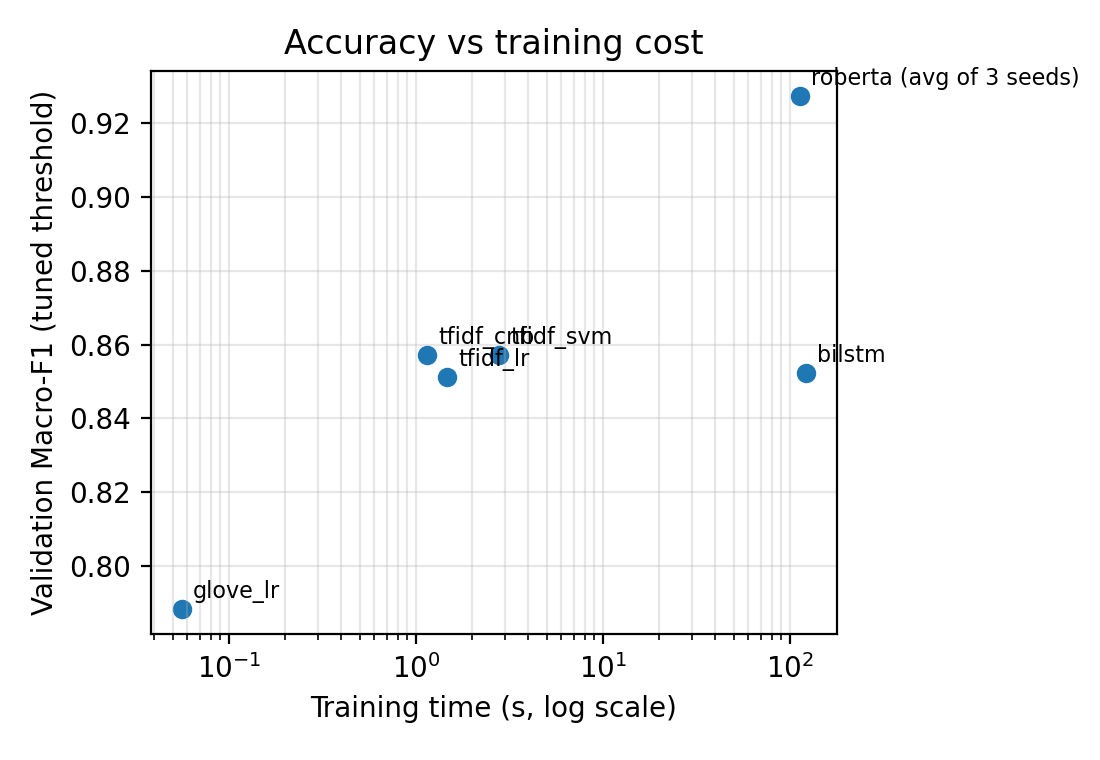
\includegraphics[width=0.62\textwidth]{f1_vs_train_time.png}
\caption{调好阈值后的验证集 Macro-F1 与训练时间（对数坐标）。对于神经网络集成，训练时间按每个 seed 报告。RoBERTa 的点使用三次预热训练的运行。}
\label{fig:g-scatter}
\end{figure}

\paragraph{实际启示。}
\begin{itemize}
  \item \textbf{标注数据少时，预训练特征更有利。} 只有 5.9k 条训练评论时，TF-IDF 必须从零学习每个 n-gram 的极性，而且验证评论中 24\% 的词类型从未在训练中出现。预训练词向量，尤其是预训练语言模型，带来了从数十亿词中学到的知识，因此对罕见词、错别字和同义改写的泛化更好。
  \item \textbf{数据量大或预算紧时，稀疏特征更有利。} TF-IDF 线性扩展、可在任何 CPU 上运行且完全可解释。当延迟、成本或可解释性比最后一个百分点更重要时，它是正确的选择，并且是很强的基线。
  \item \textbf{对领域变化的鲁棒性不同。} TF-IDF 和 GloVe 在训练时就固定了词表，而子词模型可以覆盖任何输入字符串，这对第~\ref{sec:hotel} 节中的酒店评论场景很重要。
\end{itemize}
简而言之，对这个任务而言，特征格式只会把精度改变几个点，却会把成本改变几个数量级。因此选择应当依据精度目标和可用硬件。

%=====================================================================
\section{领域迁移：无评分的酒店评论}\label{sec:hotel}

酒店评论与商品评论共享 \emph{excellent}、\emph{disappointing} 这样的通用线索，因此冻结的源域分类器是一个有用的起点。但某些特征的含义会变：\emph{small} 可以指方便的电子设备，也可以指小得让人不舒服的房间。酒店评论还会讨论服务、清洁度和位置，而且常在同一条评论里出现相互矛盾的观点。话题分布或类别比例的变化，可能使源域的决策阈值在酒店评论上校准不佳。已有的评论迁移研究为这些风险提供了证据，但在酒店评论上损失有多大，仍需要在目标领域上评估\cite{blitzer2007biographies,karouzos2021udalm}。

\paragraph{利用原始酒店文本做自适应。}
一种做法是先在无标签酒店评论上继续做掩码语言模型训练，再用带标签的商品评论训练情感分类头。另一种做法是用源域标签训练情感分类头，同时用酒店语料做联合的掩码语言模型目标，如 UDALM\cite{karouzos2021udalm}。更便宜的办法是自训练：用源域模型给无标签的酒店评论池打标签，从每个预测类别中只保留高置信度的样本，再用原有的带标签评论和对伪标签降低的权重重新训练。置信度截断应当保守，因为域偏移会产生高置信度的错误，并加剧类别不平衡。对轻量的线性模型，结构对应学习则可以利用频繁出现的共享枢轴词来连接商品和酒店的词汇\cite{blitzer2007biographies}。

\paragraph{评估。}
如果可以人工标注，就按固定的整体极性标准，独立标注约 100 条随机抽取的酒店评论。对分歧进行裁定，并记录如何处理混合或中性评论。把这个集合与无标签的自适应池分开保存。在同样的有标签评论上，用准确率、Macro-F1 和负类 F1 比较冻结的源域模型与各个自适应后的模型。凡是用酒店标签选出的阈值，都需要单独的校准集或嵌套验证流程。没有目标域标签时，可以检查 OOV 率和预测分布作为诊断，但不报告目标域准确率。

%=====================================================================
\section{噪声标签：评分不准确的酒店评论}\label{sec:noise}

题目中提到 ``the same sentiment classification problem in (g)''。我们把它理解为第~\ref{sec:hotel} 节的酒店评论项目：评论现在带有评分，但其中一些评分是错的。
因此由评分得到的训练标签是\emph{带噪声}的。

\subsection{对我们分类器的影响}

\paragraph{噪声的来源与类型。}
评论网站上的评分错误很少是均匀的\cite{song2023learning}。可以区分三种：
\begin{itemize}
  \item \emph{随机错误}，如误点或评分量表弄反，大致是\emph{对称}的。
  \item \emph{系统性错误}是\emph{类别相关}的。住客可能写了正面的文字，却因为价格或某一次事件给了低分，或者酒店得到了虚高的评分。噪声于是主要沿一个方向发生。
  \item \emph{实例相关的错误}集中在含糊、混合或带讽刺的评论上，而这些恰恰是困难样本。
\end{itemize}

\paragraph{对训练的影响。}
判别式分类器会拟合给定的标签。
过参数化的神经网络甚至能记住完全随机的标签。不过它们倾向于先学到干净的、占主导的模式，之后才去拟合噪声。
因此，在带噪声的评分上训练到收敛的微调 RoBERTa 或 BiLSTM，会逐渐吸收这些错误，决策边界和置信度估计都会受损。在干净数据上做早停可以推迟这一点，但不能避免。
带正则化的线性 TF-IDF 模型不能自由地记忆，但它的权重会以同样的方式产生偏差。
类别不平衡会放大这种损害。在 85:15 的类别比例下，每个标签以 20\% 的概率独立翻转时，被标为``负面''的评论中只有 41\% 是真正的负面，因为翻转过来的正样本比真正的负样本还多。
少数类（通常正是酒店最关心的那一类）首先受到影响。

\paragraph{对评估的影响。}
如果验证集和测试集的标签也有噪声，测得的准确率会低估真实准确率，模型选择和阈值调整也会去追逐噪声。
因此，一小批人工核实过的干净数据对下面所有改进方法都是必不可少的。

\subsection{实验：向我们的数据注入标签噪声}
为了量化这些影响，我们破坏了训练部分 5{,}909 条评论的标签，并保持 1{,}492 条验证集评论干净。
我们使用了两种噪声模型：
\begin{itemize}
  \item \emph{对称}：每个标签以 0、5\%、10\% 或 20\% 的概率翻转；
  \item \emph{正面$\to$负面}：只翻转正面标签，概率为 5\%、10\% 或 20\%，模拟``正面文字却给了低分''的情形。
\end{itemize}
基础模型是 TF-IDF（词 1--2-gram）+ LR，每种设置用 3 个 seed 重复。
方法 M1--M3 依赖在带噪训练部分上计算的 5 折折外概率 $p(x)$，所用的分组折与第~\ref{sec:data} 节相同。我们比较四种策略：
\begin{itemize}
  \item \textbf{M0，基线}：直接在带噪标签上训练。
  \item \textbf{M1，样本选择（Confident Learning）}\cite{northcutt2021confident}。对每个类别 $j$，把阈值 $t_j$ 设为标签为 $j$ 的样本上预测概率 $j$ 的均值。如果一个样本在满足 $p_k \ge t_k$ 的类别中概率最大的那个类与它的给定标签不同，就标记该样本。被标记的样本被删除，然后重新训练模型。
  \item \textbf{M2，标签修正}：当折外模型给相反类别的概率超过 0.9 时，翻转该标签。
  \item \textbf{M3，重加权}：每个样本的权重取其给定标签的折外概率。
\end{itemize}

\begin{table}[!htbp]
\centering
\caption{注入标签噪声后的验证集结果（3 个 seed 的均值 $\pm$ 标准差）。左半部分：阈值 0.5 下的 Macro-F1。右半部分：与阈值无关的 ROC-AUC。``负标签精度''指训练评论中被标为负面的那部分里，真正是负面的比例。在不加类别权重、也不调阈值的情况下，干净基线的 Macro-F1（0.789）低于 第~\ref{sec:formats} 节中调好阈值的 TF-IDF 模型（0.851）。}
\label{tab:i-noise}
\small
\setlength{\tabcolsep}{3.5pt}
\begin{tabular}{l r c cccc cccc}
\toprule
 & & 负标签 & \multicolumn{4}{c}{Macro-F1 @ 0.5} & \multicolumn{4}{c}{ROC-AUC} \\
\cmidrule(lr){4-7}\cmidrule(lr){8-11}
噪声 & 比例 & 精度 & M0 & M1 & M2 & M3 & M0 & M1 & M2 & M3 \\
\midrule
--          & 0\%  & 1.00 & .789 & \textbf{.810} & .765 & .692 & \textbf{.950} & .948 & .946 & .945 \\
对称   & 5\%  & 0.77 & .789 & \textbf{.814} & .789 & .698 & .938 & \textbf{.944} & \textbf{.944} & \textbf{.944} \\
            & 10\% & 0.60 & .772 & \textbf{.805} & .765 & .690 & .910 & .936 & .929 & \textbf{.939} \\
            & 20\% & 0.41 & .720 & \textbf{.792} & .754 & .724 & .837 & \textbf{.909} & .878 & .907 \\
正$\to$负 & 5\%  & 0.77 & .802 & \textbf{.823} & .812 & .728 & .935 & \textbf{.944} & \textbf{.944} & \textbf{.944} \\
            & 10\% & 0.63 & .806 & \textbf{.819} & .809 & .769 & .917 & .940 & .936 & \textbf{.941} \\
            & 20\% & 0.46 & .778 & \textbf{.819} & .796 & .814 & .901 & .931 & .917 & \textbf{.933} \\
\bottomrule
\end{tabular}\\[2pt]
\footnotesize Macro-F1 的标准差为 0.003--0.020，AUC 的标准差小于 0.008；完整数值见项目代码库（附录~\ref{app:code}）。
\end{table}

\begin{figure}[!htbp]
\centering
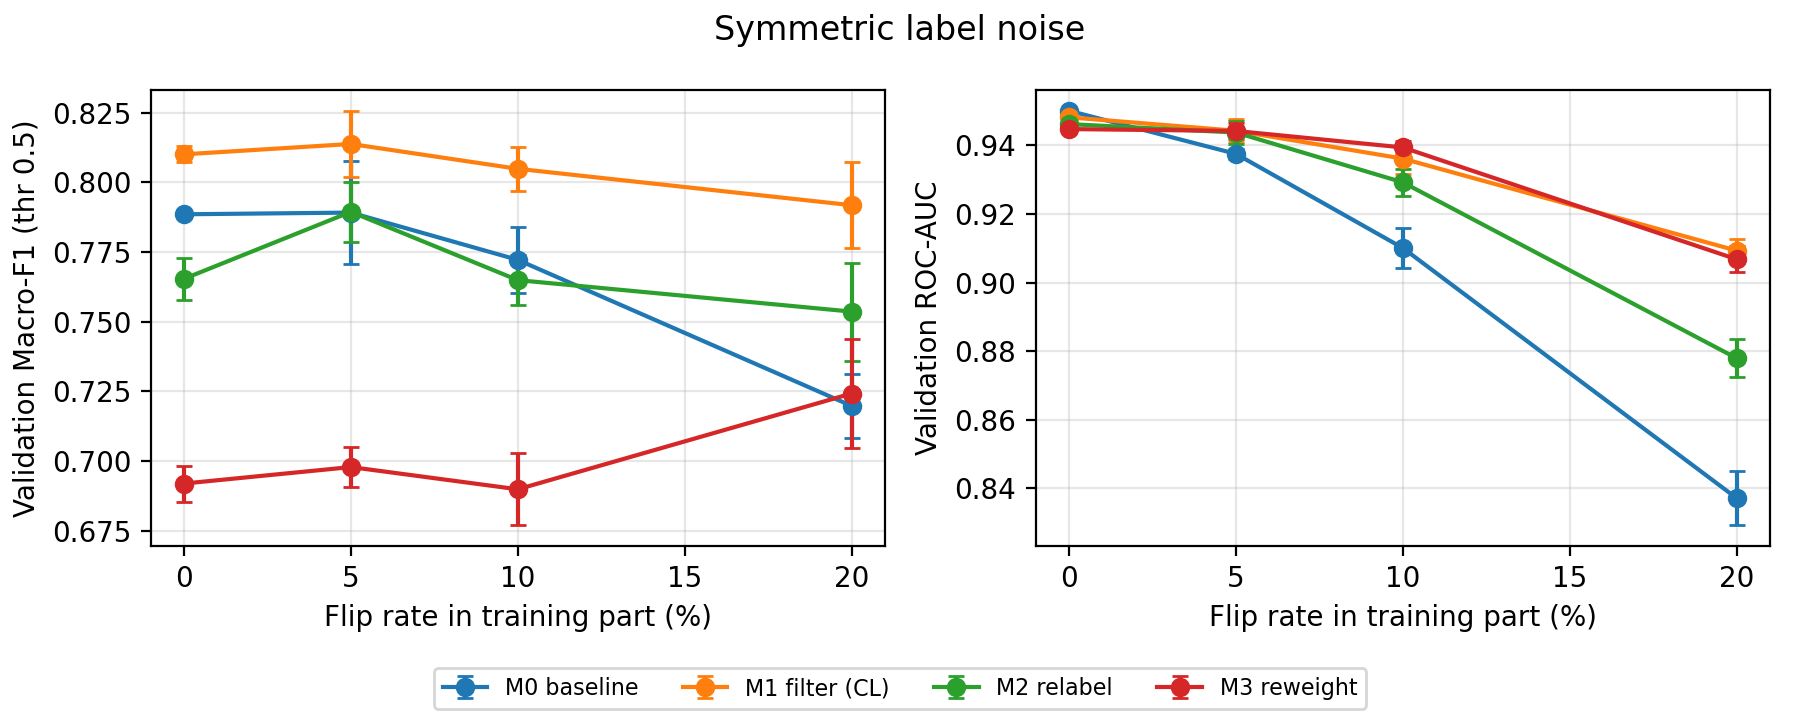
\includegraphics[width=\textwidth]{noise_symmetric.png}\\[4pt]
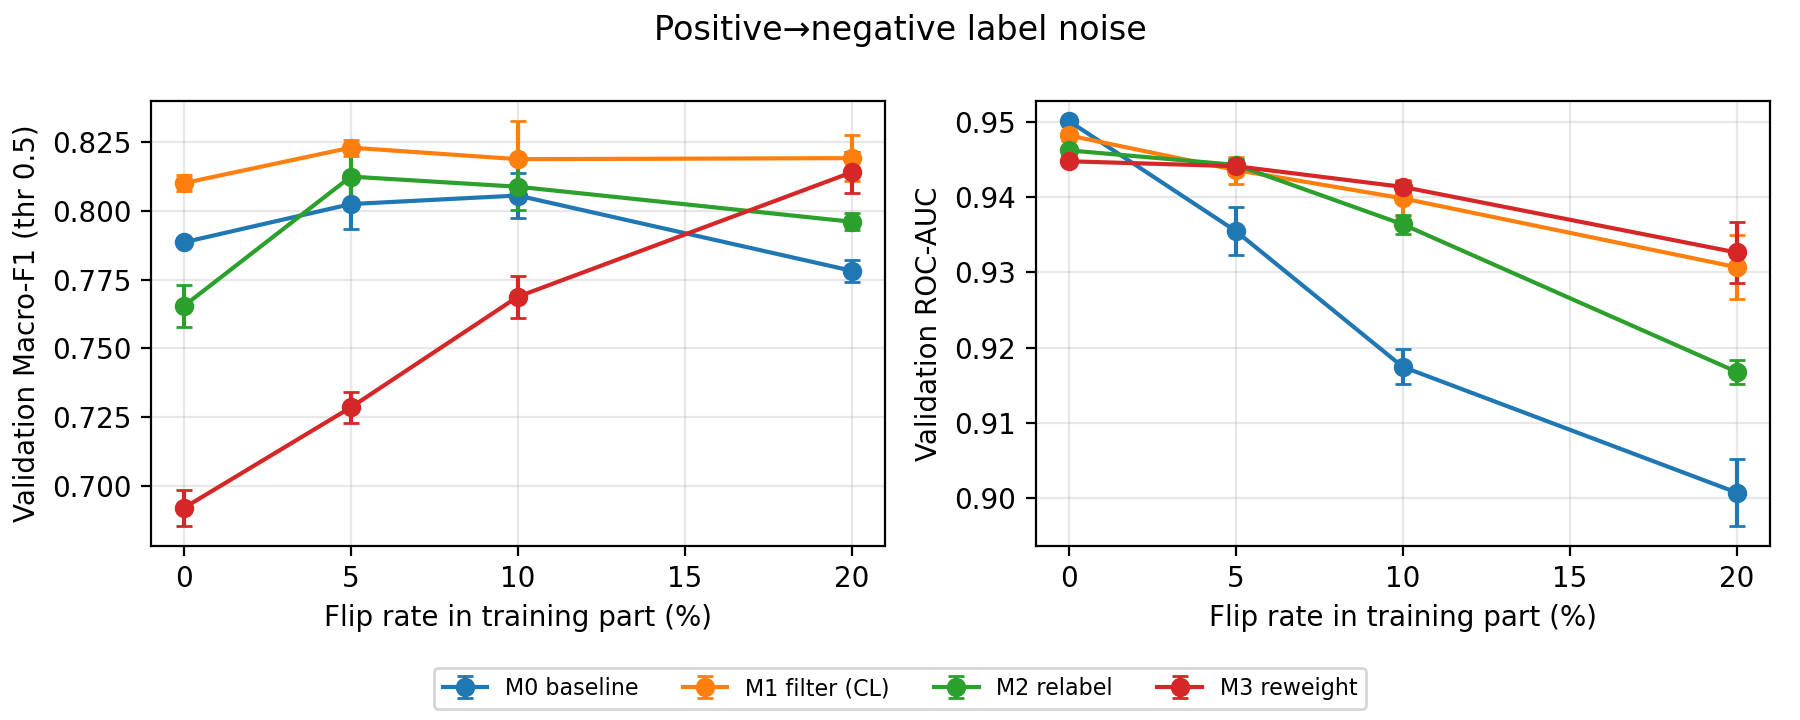
\includegraphics[width=\textwidth]{noise_pos2neg.png}
\caption{随训练标签翻转比例增加，阈值 0.5 下的验证集 Macro-F1（左）和 ROC-AUC（右）。误差线表示 3 个 seed 的 $\pm1$ 个标准差。}
\label{fig:i-noise}
\end{figure}

\paragraph{发现。}
表~\ref{tab:i-noise} 和图~\ref{fig:i-noise} 给出五点观察。
\begin{enumerate}
  \item \textbf{噪声有害，类别不平衡使其更糟。} 在 20\% 对称噪声下，基线的 AUC 从 0.950 降到 0.837，Macro-F1 从 0.789 降到 0.720。负类 F1 从 0.63 降到 0.52。
  \item \textbf{阈值 0.5 下的指标可能有误导性。} 5--10\% 的正$\to$负噪声反而使基线在 0.5 阈值下的 Macro-F1 略有\emph{上升}，尽管它的 AUC 在下降。多出来的负标签只是把决策边界推向了少数类。这就是我们同时报告 AUC 的原因，也是必须在干净数据上调阈值的原因。
  \item \textbf{样本选择（M1）是最可靠的方法。} 它在每种设置下的 Macro-F1 都最好，在 20\% 对称噪声下把 AUC 从 0.837 恢复到 0.909。它平均删除了 1{,}633 条评论，其中 44\% 确实是被翻转过的，并找出了全部被翻转标签的 61\%。即使在干净数据上，它也删掉了约 80 条困难或含糊的评论，并使 Macro-F1 提高了 0.02。
  \item \textbf{标签修正（M2）精度高但偏保守。} 它改动的标签里 83--97\% 确实是错的，但它只改了 200--280 个，所以收益有限。
  \item \textbf{重加权（M3）排序能力好，但需要重新校准。} 它的 AUC 与 M1 相当，在强的正$\to$负噪声下表现最好。但在低噪声时，它在 0.5 阈值下的 Macro-F1 很差：负面评论得到的折外置信度较低，重加权进一步压缩了少数类。如果与类别权重或阈值调整结合，这一弱点就会消失。
\end{enumerate}
这些结果来自合成噪声、线性模型和单个验证划分。它们显示了问题的规模以及各类策略的相对表现，而不是在真实酒店评分上应预期的提升幅度。

\subsection{改进算法的三种方法}
下面三类方法遵循近期综述 Song 等人\cite{song2023learning} 的分类体系，这里提到的各个具体方法在该综述中有详细介绍。
\begin{enumerate}
  \item \textbf{抗噪声损失与损失修正。} 用对错误标签的惩罚更轻的损失函数替代普通交叉熵。可选的包括：在交叉熵与抗噪的 MAE 之间插值的广义交叉熵（GCE）；对称交叉熵；以及标签平滑。
  当噪声是类别相关的（例如``正面文字却给了低分''）时，还可以估计 $2\times2$ 的噪声转移矩阵 $T$，并通过它修正损失（前向/后向修正）。$T$ 可以由一小批干净数据估计。
  这些方法只改变我们 RoBERTa 微调所用的损失函数，不增加额外成本。

  \item \textbf{样本选择与数据清洗。} 利用网络先拟合干净样本这一事实，小损失样本更可能是标注正确的。
  Co-teaching 训练两个网络，让每个网络只用对方选出的小损失样本更新。Confident Learning 利用折外概率估计带噪标签与真实标签的联合分布，然后剪除或排序可疑样本\cite{northcutt2021confident}；这就是我们的 M1，也是我们实验中最好的方法。
  被标记的评论也可以交给标注人员复核，而不是直接丢弃。

  \item \textbf{标签修正与半监督学习。} 与其丢弃可疑样本，不如修正它们或降低其权重。我们的 M2 和 M3 是简单版本。
  DivideMix 对每个样本的损失拟合两成分混合模型，以区分可能干净与可能带噪的评论。然后把带噪的评论当作\emph{无标签}数据，用 MixMatch 式的半监督学习同时利用两部分数据训练。
  对于酒店评论，文本本身是第二个独立的信号。零样本模型（例如我们的 RoBERTa 分类器或大语言模型）可以对照文本检查每个评分，两者结合可以得到修正后的标签。
\end{enumerate}

\paragraph{针对酒店项目的建议流程。}
\begin{enumerate}
  \item 人工核实几百条评论，得到一个干净的开发集，并用它估计噪声比例和转移矩阵 $T$。
  \item 用抗噪声损失（GCE 或标签平滑）微调预训练 Transformer，并在干净集上做早停。
  \item 在折外预测上运行 Confident Learning；对被标记的评论进行修正标签或删除，不确定的送交标注人员。
  \item 重新训练，可选地对存疑部分使用 DivideMix 式的半监督学习，并在干净集上调决策阈值。
\end{enumerate}

%=====================================================================
\section{结论}\label{sec:conclusion}
我们在同一个无泄漏的验证划分上，比较了稀疏 TF-IDF 特征、静态 GloVe 词向量和微调的 RoBERTa 子词表示。
三个 seed 的 RoBERTa 集成表现最好，在验证集调好的阈值下准确率为 0.962、Macro-F1 为 0.927，明显领先于 TF-IDF 加线性 SVM（0.930 和 0.857）。
BiLSTM 只与 TF-IDF 持平，训练时间却约为其 80 倍；平均 GloVe 向量最弱（Macro-F1 为 0.788）。
因此对这个任务而言，特征格式只让精度改变几个点，却让成本改变几个数量级。
微调还对随机种子敏感：不做学习率预热时，三次运行中有一次崩溃为常数预测，加上预热后问题消失。

这些结论有局限。
所有模型选择都基于同一个验证划分，其中只有 218 条负面评论，因此不应过度解读微小差异。
第~\ref{sec:analysis} 节的样本分析考察的是初始集成而不是最终集成，噪声实验使用的是合成噪声和线性模型。
下一步自然是：对最终集成重做误差分析，在真实的酒店评论上评估模型，并用 RoBERTa 测试抗噪声损失。

\appendix
\section{代码与可复现性}\label{app:code}
全部代码、数据划分和输出都在提交的压缩包中。主要文件如下：
\begin{itemize}
  \item \texttt{README.md}：安装说明以及复现每项结果的命令；
  \item \texttt{src/common.py}：数据读取、共享的验证划分、指标、阈值选择以及 \texttt{submission.csv} 的写出；
  \item \texttt{src/tfidf\_models.py}、\texttt{src/tfidf\_dim\_study.py} 和 \texttt{src/resource\_table.py}：TF-IDF 模型、维度研究和资源表（第~\ref{sec:hparams} 节和第~\ref{sec:formats} 节）；
  \item \texttt{src/noise\_exp.py}：标签噪声实验（第~\ref{sec:noise} 节）；
  \item \texttt{src/glove\_bilstm.py}：GloVe 特征、平均词向量分类器和 BiLSTM；
  \item \texttt{src/transformer\_ft\_warmup.py}、\texttt{src/transformer\_ft.py} 和 \texttt{src/ensemble.py}：RoBERTa 微调与最终预测；
  \item \texttt{splits/val\_idx.npy}：共享的验证集下标；
  \item \texttt{outputs/<model>/}：验证集和测试集概率、指标和超参数日志（例如 \texttt{outputs/bilstm/hparam\_log.csv}）；
  \item \texttt{outputs/noise\_exp/summary.csv}：完整的噪声实验结果。
\end{itemize}
随机种子是固定的（神经模型为 42、43 和 44），因此保存的输出可以重新生成。

\bibliographystyle{unsrtnat}
\bibliography{../refs}
\end{document}
